%%%%%%%%%%%%%%%%%%%%%%%%%%%%%%%%%%%%%%
%%%%%%%%%%%%%%%%%%%%%%%%%%%%%%%%%%%%%%
%%%%%%%%%%%%%%%%%%%%%%%%%%%%%%%%%%%%%%
%%%%%%%%%%%%%%%%%%%%%%%%%%%%%%%%%%%%%%
%%%%%%%%%%%%%%%%%%%%%%%%%%%%%%%%%%%%%%
\section{Introduction}
Statistical machine learning is a subject that aims to build and train algorithms, that analyse large amount of data, and make predictions for the future, which are computed by using established statistical models, and tools from functional analysis. This is a project in supervised, statistical machine learning, where several models were created, and trained, in order to analyse which one of them gives best prediction for the project "Do we need more bikes", where we want to understand, and predict if there is a high, or low demand of city bikes in the public transportation of Washington, a project by the District Department of Transportation in Washington D.C..

The data set used for training our models, consist of 15 variables, containing quantitative/qualitative data. We developed several models, and evaluated them with cross-validation, in order to understand which algorithm gives the best prediction. 



%%%%%%%%%%%%%%%%%%%%%%%%%%%%%%%%%%%%%%
%%%%%%%%%%%%%%%%%%%%%%%%%%%%%%%%%%%%%%
%%%%%%%%%%%%%%%%%%%%%%%%%%%%%%%%%%%%%%
%%%%%%%%%%%%%%%%%%%%%%%%%%%%%%%%%%%%%%
%%%%%%%%%%%%%%%%%%%%%%%%%%%%%%%%%%%%%%
\section{Data analysis}

















%%%%%%%%%%%%%%%%%%%%%%%%%%%%%%%%%%%%%%
%%%%%%%%%%%%%%%%%%%%%%%%%%%%%%%%%%%%%%
%%%%%%%%%%%%%%%%%%%%%%%%%%%%%%%%%%%%%%
%%%%%%%%%%%%%%%%%%%%%%%%%%%%%%%%%%%%%%
%%%%%%%%%%%%%%%%%%%%%%%%%%%%%%%%%%%%%%
\section{Theoretical Background}


\subsection{Mathematical Overview of the Models}
    \subsubsection{Logistic Regression}
    The backbone of logistic regression is linear regression, i.e. finding the least-squares solution to an equation system \begin{equation}
        X\theta = y
    \end{equation}
    given by the normal equations \begin{equation}
        X^TX \theta = X^Ty
    \end{equation}
    where $X$ is the training data matrix, $\theta$ is the coefficient vector and $b$ is the training output. The parameter vector is then used in the sigmoid function: \begin{align}
        \sigma(z) &= \frac{e^{z}}{1+e^{z}}: \; \mathbb{R}\to [0,1],\\
        z &= x^T \theta,
    \end{align}
    where $x$ is the testing input. This gives a statistical interpretation of the input vector. In the case of a binary True/False classification, the value of the sigmoid function then determines the class.

\subsubsection{Random forest}

The random forest method is a based upon decision trees, i.e. dividing the data point into binary groups based on Gini-impurity, entropy or classification error, Gini being the most common. 
These divisions are then used to create a binary tree shown in figure \ref(Tree) and where thee leaf-nodes are used to classify the target variables bases on the input. 
As of itself the dicition tree tends to have unsatisfying results which leads to methodes like random forest that boost its accuracy.

    %%%%%%%%%%%%%%%%%%%%%%%%%%%%%%%%
    %%%%%%%%%%%%%%%%%%%%%%%%%%%%%%%%
    %%%%%%%%%%%%%%%%%%%%%%%%%%%%%%%%
    %%%%%%%%%%%%%%%%%%%%%%%%%%%%%%%%
    %%%%%%%%%%%%%%%%%%%%%%%%%%%%%%%%
    \subsubsection{Non-parametric method: k--Nearest Neighbour}
        \emph{$k$-- Nearest Neighbour}($k$--NN) is a distance based method that takes a $k$ amount of points from the training data set, called \emph{neighbours}, computes the distance between them, then assumes that the predicted value $\hat{y}(x_{*})$ follows the trend of the $k$-- nearest neighbours. Since $k$--NN uses the training data explicitly it is also called a \emph{nonparametric} method.

    The $k$--NN method can be divided into several subcategories, inter alias \emph{classification} $k$--NN method, \emph{regression}  $k$--NN method. In this project, we are using the classification method, since we are trying to predict in which of the two classes low, or high demand, the given, and predicted data points belong.

    The classification  $k$--NN algorithm evaluates $\hat{y}(x_{*})$ by computing the most frequently occurring class among the $k$ nearest neighbours. Here, we try to identify whether a data point belong to the high demand-class. Denote $c=$ high demand class. For simplicity, assume Euclidean ambiance. Then
        \begin{equation*}
            \hat{y}(x_*) = \arg \max_{c}  \sum_{n \in \mathbb{N}} \chi_{(y_i = c)} ,
        \end{equation*}
    where $y_i$ is the class of the nearest neighbour,  $\chi$ is the characteristic function 
        \begin{equation*}
            \chi_{(y_i = c)} = 
            \begin{cases}
                1 \qquad \text{if } y_n = c, \\
                0 \qquad \text{otherwise}.
                
            \end{cases}
        \end{equation*}
    It is very common to use a weighted sum to predict the next value, i.e.
        \begin{equation*}
            \hat{y}(x_*) =  arg \max_{c}  \sum_{n \in \mathbb{N}} \frac{\chi_{(y_n = c)}}{d(x, x_n)},
        \end{equation*}
    where $d$ is the standard Euclidean metric, computing the distance between an input $x$, and a neighbour $x_n$. 

    When using this model it is important to choose an optimal $k$--value. There are several tests for this, here we implement \emph{uniform weighting}, and \emph{distance weighting}. The first algorithm creates a $k$--NN model for each new $k \in [1, 500]$, and trains the model with uniform weights, i.e. the contribution of all neighbours is equal. Similarly, the latter trains a $k$--NN classifier for each $k \in [1, 500]$, with the difference that it uses distance based weighting, i.e. closer neighbours have greater influence. After testing different upper boundaries for $k$, the two models gave good results in the interval $[1,500]$, see Figure \ref{fig:kNN_comparison}. From the figures, we can see that the second test gives a better value for $k$, since the plot follows smoother trend, in comparison to the uniform weighting test, which makes it easier to identify an optimal $k$ value ($k = 120$). Moreover, the distance weighting algorithm is providing results for larger values of $k$, that is for $k \in [1, 400)$ before the curve converges, while the uniform weighting algorithm converges earlier, when $k = 290$. This means that for large $k$, both test algorithms make prediction based on the most common class in the data set, instead of making prediction based on the behaviour of the neighbours. Thus for sufficiently large $k$, for any given data point, the model will consider unnecessarily large amount of neighbours, and the prediction will be evaluated to belong to the most frequent class. Since the distance weighting has a larger range of $k$--value, it should be more trustworthy.
    
    \begin{figure}[htbp]
        \centering
        \begin{subfigure}{0.45\textwidth}
            \centering
            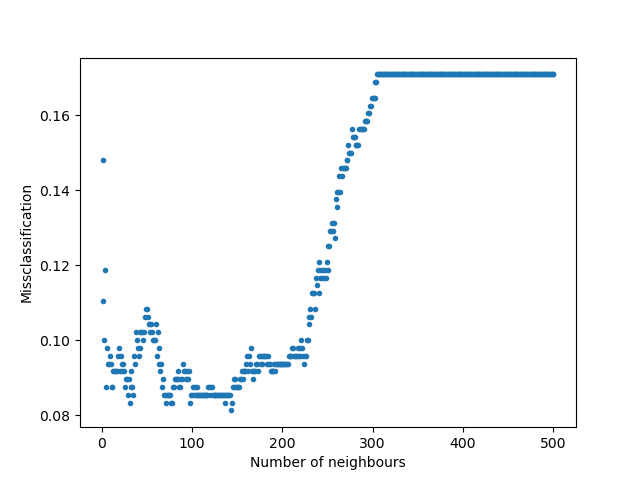
\includegraphics[width=\textwidth]{k-valueTest1ngh500.png}
            \caption{Uniform distance test for $k$.}
            \label{fig:kNN_fig1}
        \end{subfigure}
        \hfill
        \begin{subfigure}{0.45\textwidth}
            \centering
            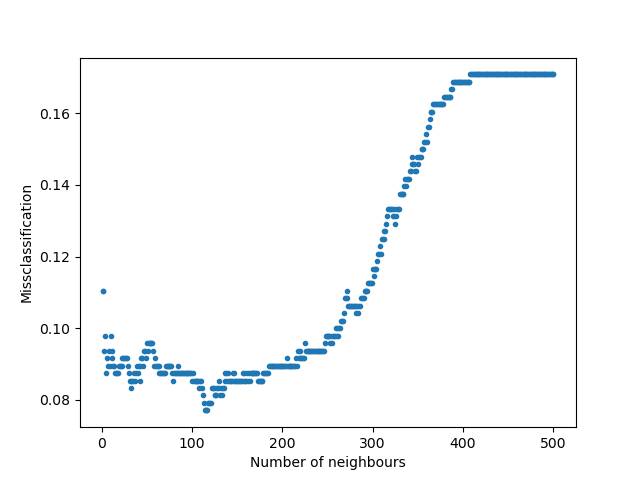
\includegraphics[width=\textwidth]{k-valueTest2ngh500.png}
            \caption{Weighted distance test for $k$.}
            \label{fig:kNN_fig2}
        \end{subfigure}
        \caption{Test for choosing an optimal $k$--value.}
        \label{fig:kNN_comparison}
    \end{figure}

    With the $k = 280$, the

    







    %%%%%%%%%%%%%%%%%%%%%%%%%%%%%%%%
    %%%%%%%%%%%%%%%%%%%%%%%%%%%%%%%%
    %%%%%%%%%%%%%%%%%%%%%%%%%%%%%%%%
    %%%%%%%%%%%%%%%%%%%%%%%%%%%%%%%%
    %%%%%%%%%%%%%%%%%%%%%%%%%%%%%%%%
    \subsection{Input Data Modification}
    \label{sec:input data modification}
    By plotting the data and analyzing the .csv file, some observations were made. The different inputs were then changed accordingly:
    \begin{itemize}
        \item \emph{Kept as-is}: \texttt{weekday}, \texttt{windspeed}, \texttt{visibility}, \texttt{temp}
        \item \emph{Modified}:
        \begin{itemize}
            \item \texttt{month} - split into two inputs, one cosine and one sine part. This make the new inputs linear and can follow the fluctuations of the year. The original input was discarded.
            \item \texttt{hour\_of\_day} - split into three boolean variables: \texttt{demand\_day}, \texttt{demand\_evening}, and \texttt{demand\_night}, reflecting if the time was between 08-14, 15-19 or 20-07 respectively. This was done because plotting the data showed three different plateaues of demand for the different time intervals. The original input was discarded.
            \item \texttt{snowdepth}, \texttt{precip} were transformed into booleans, reflecting if it was raining or if there was snow on the ground or not. This was done as there was no times where demand was high when it was raining or when there was snow on the ground.
        \end{itemize} 
        \item \emph{Removed}: \texttt{cloudcover}, \texttt{day\_of\_week}, \texttt{snow}, \texttt{dew}, \texttt{holiday}, \texttt{summertime}. These were removed due to being redundant (e.g. \texttt{summertime}), not showing a clear trend (e.g. \texttt{cloudcover}), giving a worse score when used, or all three (e.g. \texttt{day\_of\_week}).
    \end{itemize}